%========================================================================================
% Latex-Beamer-Template
% TU Dortmund, Informatik Lehrstuhl VII
%========================================================================================
\documentclass[10pt]{beamer}

\usetheme{tufi}
\usepackage{amsmath,amssymb}
%\usepackage{flafter}
\usepackage{subfig}

\usepackage{wasysym}
\usepackage[ngerman]{babel}
\usepackage[utf8]{inputenc}
\usepackage{amsmath,amsfonts,amssymb}
\usepackage{graphicx}
\usepackage[T1]{fontenc}
\usepackage{verbatim}
\usepackage[babel,german=quotes]{csquotes}
\usepackage{array}
\usepackage{multirow}
\usepackage{rotating}
\usepackage{pgfpages}
\usepackage[plain,section]{algorithm}
\usepackage{algorithmic}
\usepackage{listings}

\lstdefinestyle{C++}
{
language=C++,
backgroundcolor=\color{BrightGray},
keywordstyle=\texttt\bfseries,  %\color{TUGreen}\bfseries,
commentstyle=\color{DarkGray},
stringstyle=\color{red},
showstringspaces=false,
basicstyle=\small\color{black},
numbers=left,
captionpos=b,
tabsize=4,
breaklines=true
}

\resetcounteronoverlays{algorithm}

\renewcommand{\algorithmicrequire}{\textit{Eingabe:}}
\renewcommand{\algorithmicensure}{\textit{Ausgabe:}}
\floatname{algorithm}{Algorithmus}
\renewcommand{\listalgorithmname}{Algorithmenverzeichnis}
\renewcommand{\algorithmiccomment}[1]{\color{grau}{// #1}}
\usepackage{tabularx}

\usepackage[backend=biber]{biblatex}
\bibliography{Literatur.bib}

\newcommand\tabrotate[1]{\begin{turn}{90}\rlap{#1}\end{turn}}
\newcommand\MyBox[2]{
  \fbox{\lower0.75cm
    \vbox to 1.7cm{\vfil
      \hbox to 1.7cm{\hfil\parbox{1.4cm}{#1\\#2}\hfil}
      \vfil}%
  }%
}

%========================================================================================
% Hier Vortragstitel, Autor und Vortragsdatum eintragen
\pdfinfo
{
  /Title       (Zeit-Effizientes Training von Convolutional Neural Networks)
  /Creator     (TeX)
  /Author      (Jessica Bühler)
}


\title{Masterarbeit -- Zeit-Effizientes Training von Convolutional Neural Networks}
\author{Jessica Bühler}
\date{\today}
%========================================================================================

\begin{document}

\frame{\titlepage}

\begin{frame}
 \begin{figure}[h]
 \centering
 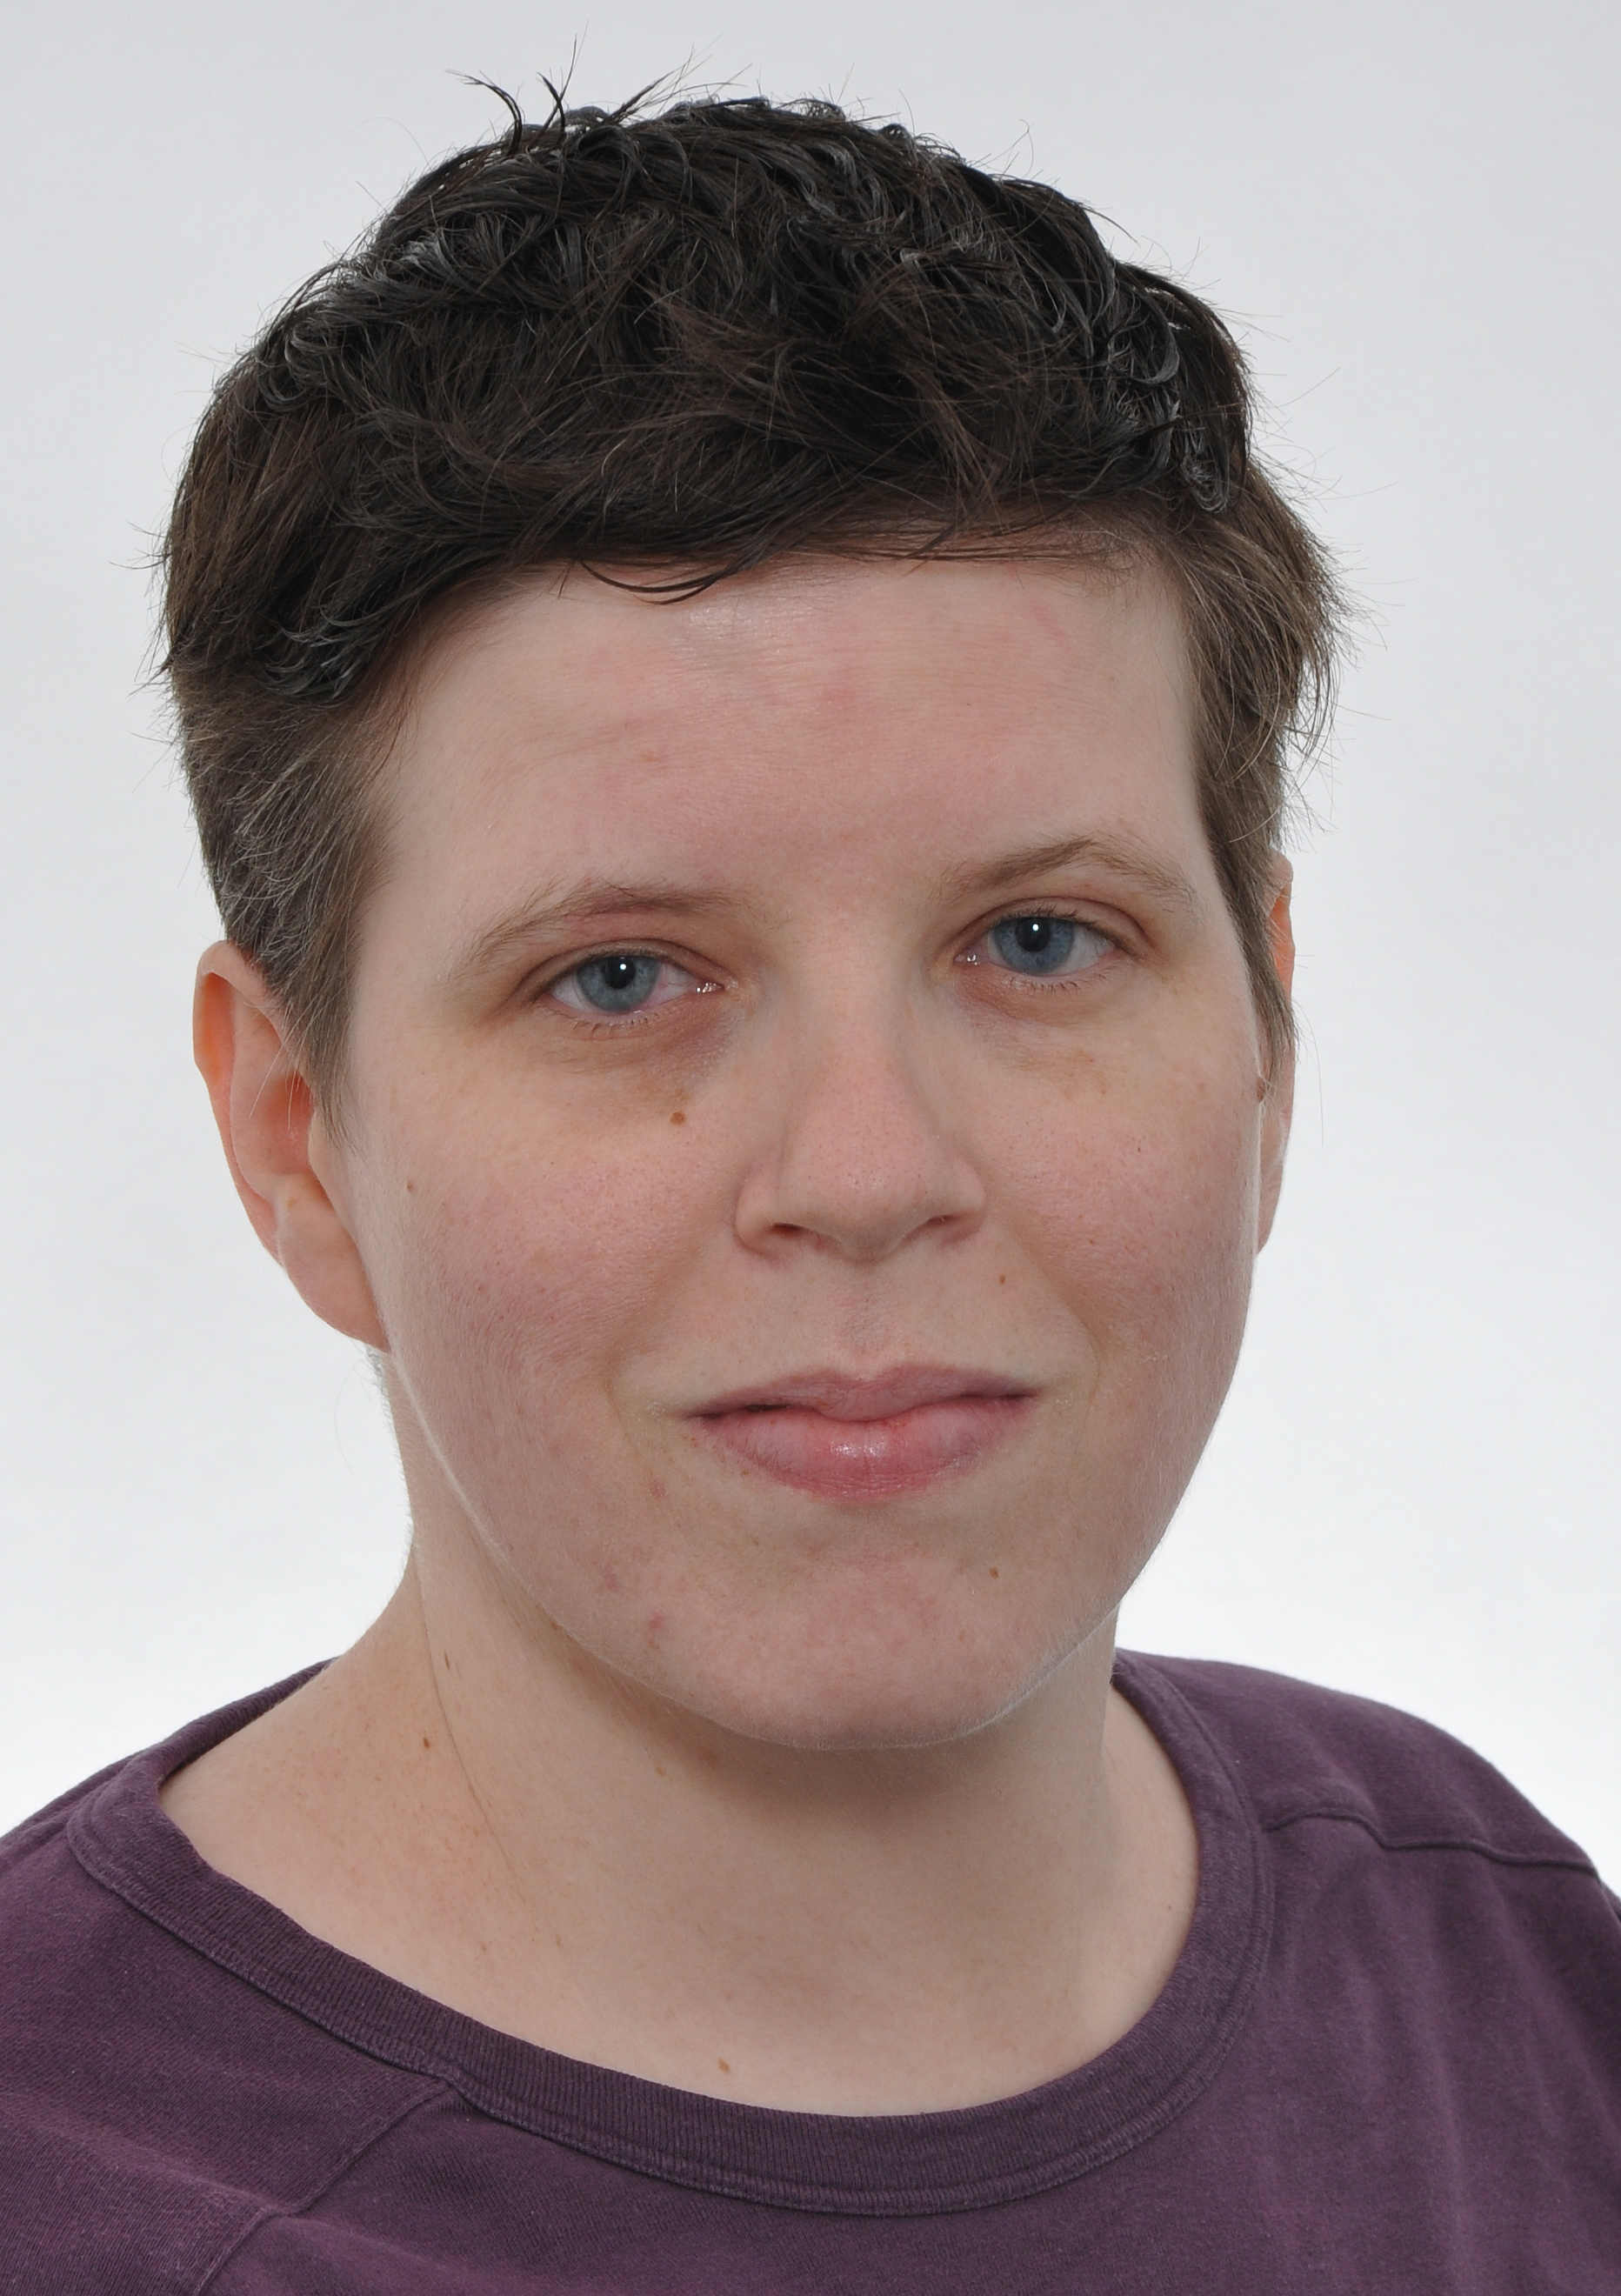
\includegraphics[width=0.4\textwidth]{images/Passbild_Buehler.jpg}
 % Passbild_Buehler.jpg: 1864x2640 px, 300dpi, 15.78x22.35 cm, bb=0 0 447 634
\end{figure}

 
\end{frame}



\AtBeginSection[]
{
  \frame<handout:0>[allowframebreaks]
  {
    \frametitle{Übersicht}
    \tableofcontents[currentsection,hideallsubsections]
  }
}

\AtBeginSubsection[]
{
  \frame<handout:0>[allowframebreaks]
  {
    \frametitle{Übersicht}
    \tableofcontents[sectionstyle=show/hide,subsectionstyle=show/shaded/hide]
  }
}

\newcommand<>{\highlighton}[1]{%
  \alt#2{\structure{#1}}{{#1}}
}

\newcommand{\icon}[1]{\pgfimage[height=1em]{#1}}


%=Inhalt=================================================================================
\section{Einleitung}


\begin{frame}{Ausgangssituation}
Gegeben: Unbekannter Datensatz aus Bildern, mit gelabelten Trainingsdaten und ungelabelten Testdaten

Aufgabe:
\begin{figure}[h]
 \centering
 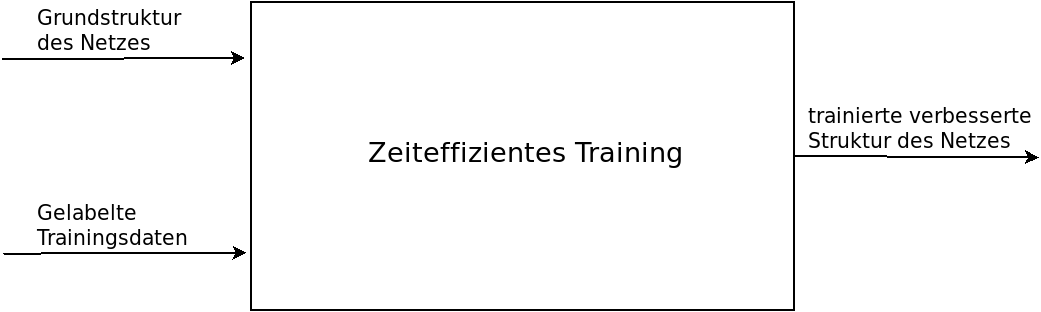
\includegraphics[width=0.8\textwidth]{images/problem.png}
 % problem.png: 1041x312 px, 72dpi, 36.72x11.01 cm, bb=0 0 1041 312
\end{figure}


\end{frame}


\begin{frame}{Verwendete Architektur I}
\begin{figure}[h]
 \centering
 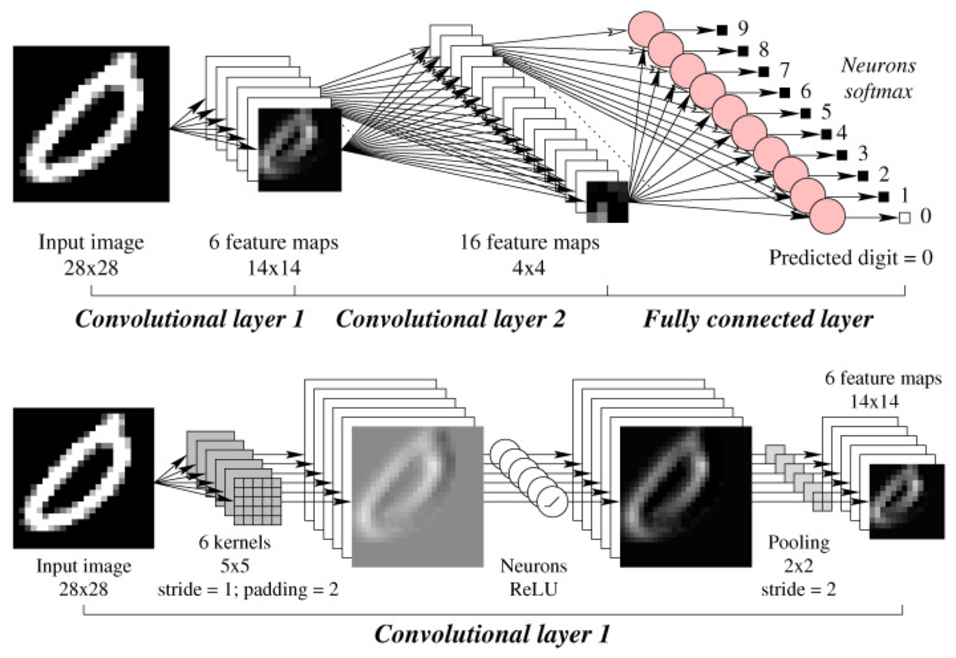
\includegraphics[width=0.8\textwidth]{images/cnn.pdf}
 % cnn.pdf: 0x0 px, 300dpi, 0.00x0.00 cm, bb=
\end{figure}
\end{frame}


\begin{frame}{verwendete Architektur II}
\begin{figure}[]
   \begin{minipage}[b]{.4\linewidth} % [b] => Ausrichtung an \caption
      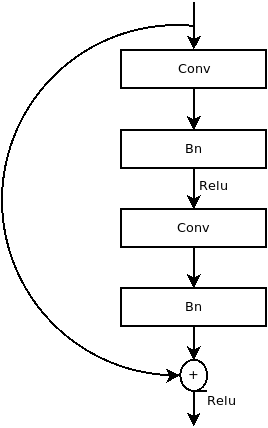
\includegraphics[width=0.8\linewidth]{images/Basisblock.png}
      \caption{Basisblock}
   \end{minipage}
   \hspace{.1\linewidth}% Abstand zwischen Bilder
   \begin{minipage}[b]{.4\linewidth} % [b] => Ausrichtung an \caption
      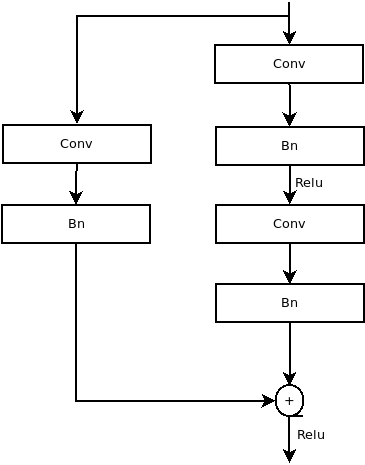
\includegraphics[width=0.8\linewidth]{images/Ubergangsblock.png}
      \caption{Übergangsblock}
   \end{minipage}
   \caption{Grafische Darstellung Basis- und Übergangsblock}
\end{figure}
\end{frame}


\begin{frame}{Bisherige Arbeiten zum Thema}
\begin{itemize}
 \item Automatische Architektursuche mit großem Suchraum
 \begin{itemize}
    \item DVolver 
 \end{itemize}
 \item Architektursuche währenddem Trainieren
 \begin{itemize}
    \item MorphNet
 \end{itemize}
\end{itemize}
\end{frame}

\section{weiteres Vorgehen}

\begin{frame}{Übersicht}
    \tableofcontents
\end{frame}


\begin{frame}{Quelle des verwendeten Codes}
 \begin{itemize}
  \item MorphNet
  \item PruneTrain
  \begin{itemize}
    \item ohne Anpassung der Batchgröße:
    \item mit zusätzlicher Anpassung der Batchgröße: eigene Implementation
  \end{itemize}
  \item Net2Net: eigene Implemetation
 \end{itemize}
\end{frame}




\begin{frame}{Baseline-Netz}
 \begin{figure}
     \centering
     \subfloat[][]{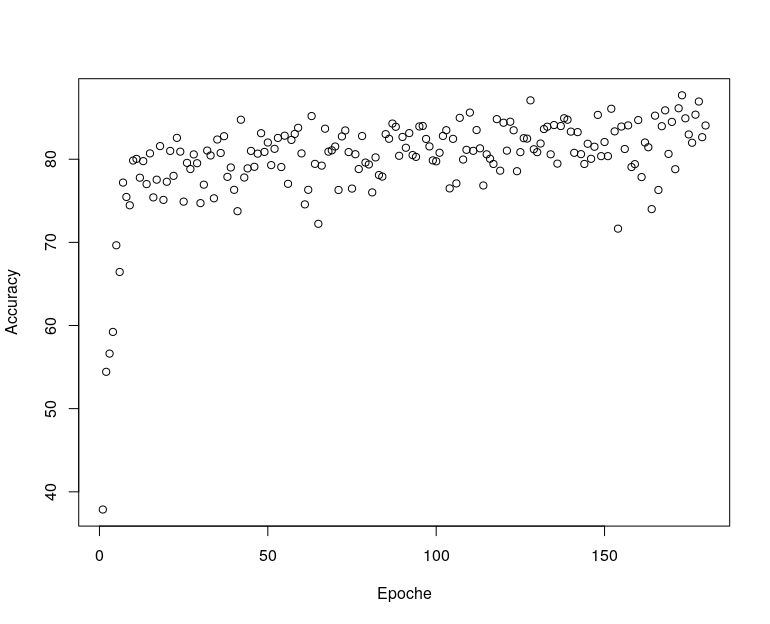
\includegraphics[width=.49\textwidth]{images/BaseAcc1.png}\label{abb:baseAcc1}}
     \subfloat[][]{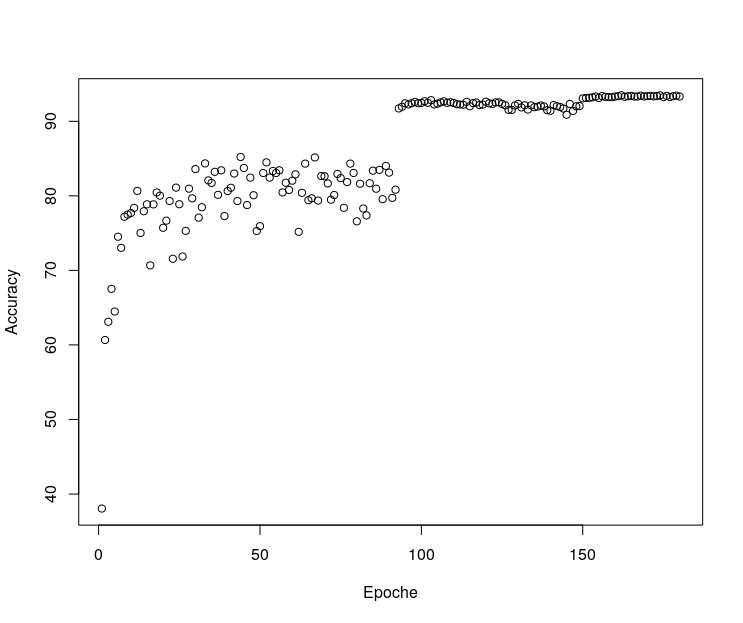
\includegraphics[width=.49\textwidth]{images/BaseAcc.png}\label{abb:baseAcc2}}
     \caption{Vergleich zwischen (a) Baseline-Netz ohne Anpassung der Lernrate und (b) Baseline-Netz mit Anpassung der Lernrate in Epoche 93 und 150.}
     \label{abb:BaseAcc}
\end{figure}

\end{frame}



\section{MorphNet}


\begin{frame}{Übersicht über MorphNet}
\begin{itemize}
 \item Morphnet vergrössert und verkleinert konkurrierend das Netz um die besten Hyperparameter zu finden
\end{itemize}
\end{frame}

\begin{frame}
\begin{algorithm}[H]
\begin{algorithmic}[1]
\STATE Trainiere das Netz um $\mathcal{W}^{\ast}=\underset{\mathcal{W}}{arg min}\; \text{Loss-Funktion des CNN} + \lambda \cdot \text{Nebenbedingung, die die Breite des Netzes minimiert}$
\STATE Finde die neue Breite $\mathcal{C}_{1:J}^{\prime}$, die durch 1. errechnet wurde
\STATE Finde das größte $\omega$, so dass $\mathcal{F}(\omega \cdot \mathcal{C}_{1:J})\leq \zeta$ gilt
\STATE Wiederhole ab 1. so häufig wie gewünscht mit $\mathcal{C}_{1:J} = \mathcal{C}_{1:J}^{\prime}$
\ENSURE $\omega \cdot \mathcal{C}_{1:J}$
\end{algorithmic}
\end{algorithm}
\end{frame}

\begin{frame}[fragile]
\begin{figure}
\begin{verbatim}   
BasicBlock(
    (0): Conv2d(76, 5, kernel_size=(3, 3), stride=(1, 1), 
    padding=(1, 1))
    (1): BatchNorm2d(5, eps=1e-05, momentum=0.1, affine=True, 
    track_running_stats=True)
    (2): ReLU(inplace=True)
    (3): Conv2d(5, 76, kernel_size=(3, 3), stride=(1, 1), 
    padding=(1, 1))
    (4): BatchNorm2d(76, eps=1e-05, momentum=0.1, affine=True, 
    track_running_stats=True))
\end{verbatim}
\caption{Struktur eines Basisblocks als Ergebnis von MorphNet 2}
\label{abb:verb2}
\end{figure}

\end{frame}


\begin{frame}[fragile]
 \begin{figure}
\begin{verbatim}
BasicBlock(
    (0): Conv2d(76, 76, kernel_size=(3, 3), stride=(2, 2),
    padding=(1, 1))
    (1): BatchNorm2d(76, eps=1e-05, momentum=0.1, affine=True,
    track_running_stats=True)
    (2): ReLU(inplace=True)
    (3): Conv2d(76, 76, kernel_size=(3, 3), stride=(1, 1), 
    padding=(1, 1))
    (4): BatchNorm2d(76, eps=1e-05, momentum=0.1, affine=True, 
    track_running_stats=True))
\end{verbatim}
\caption{Struktur eines Basisblocks als Ergebnis von MorphNet 1}
\label{abb:verb1}
\end{figure}
\end{frame}


\begin{frame}{Ergebnis der MorphNet Evaluierung}
 \begin{itemize}
  \item Bei der gegebenen Struktur 
  \item und den vorgegebenen Ressourcen
 \end{itemize}
 ist keine signifikante Verbesserung möglich.
 
 Nachteile von MorphNet:
 \begin{itemize}
  \item es ist nicht möglich, die Tiefe des Netzes zu verändern
 \end{itemize}
\end{frame}

\section{PruneTrain}
\begin{frame}{Übersicht über PruneTrain I}
 \begin{itemize}
  \item Soll den Verkleinerungsoperator von MorphNet ersetzen
  \item 
 \end{itemize}
\begin{equation*}
GL(\mathcal{W})=\sum_{j=1}^{J} \left( \sum_{c_j=1}^{C_j} || W_{j} (c_j,:,:,:) ||_2 + \sum_{k_j=1}^{K_j} || W_{j}(:,k_j,:,:)||_2 \right)
 \label{equ:PTloss}
\end{equation*}

\end{frame}

\begin{frame}{Übersicht über PruneTrain II}
\begin{figure}[h]
 \centering
 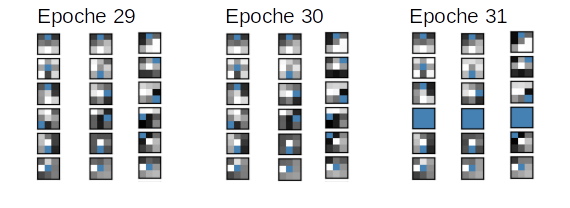
\includegraphics[width=0.8\textwidth]{images/union.png}
 % union.png: 570x208 px, 96dpi, 15.08x5.50 cm, bb=0 0 427 156
 \caption{Grafische Darstellung des Prunings des ResNets}
\end{figure}
\end{frame}


\begin{frame}{Evaluierung von PruneTrain bei Veränderung der Batchgröße der Batchgröße}
 
 \begin{figure}
     \centering
     \subfloat[][]{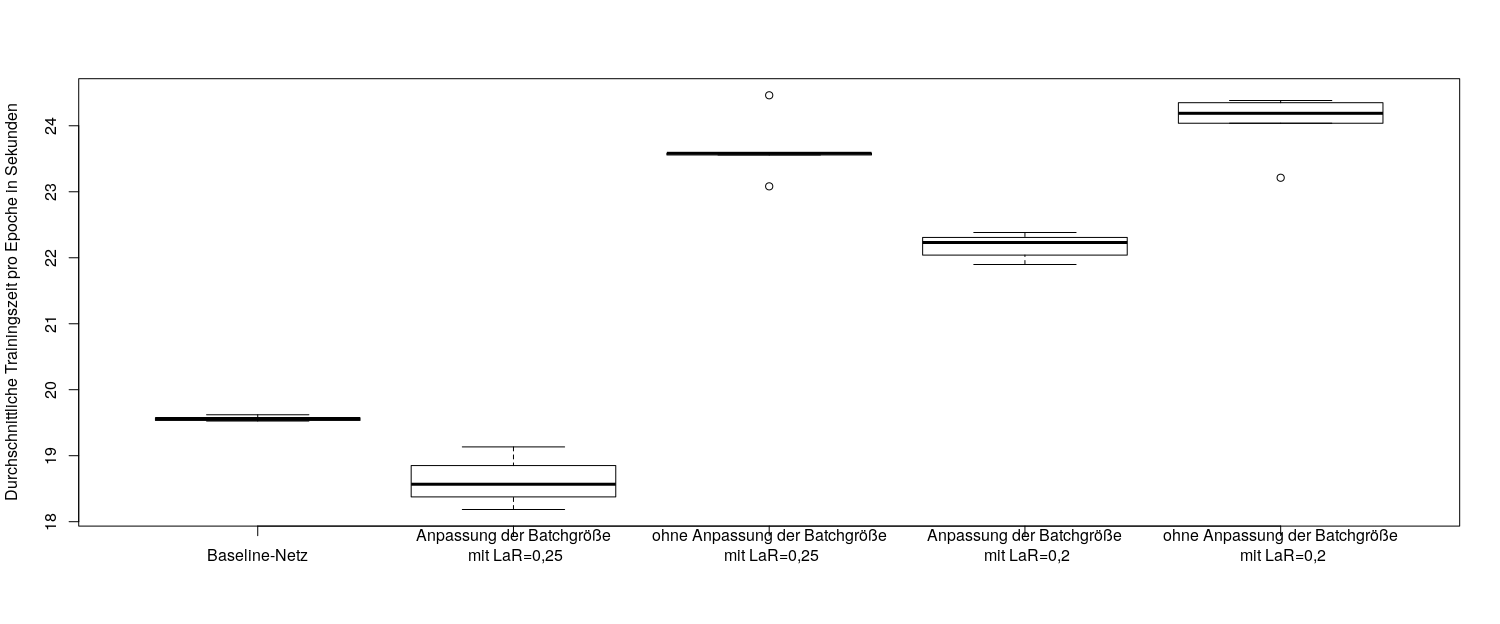
\includegraphics[width= .75\textwidth]{images/bSize1.png}\label{abb:bSize1}}
     \hfill
     \subfloat[][]{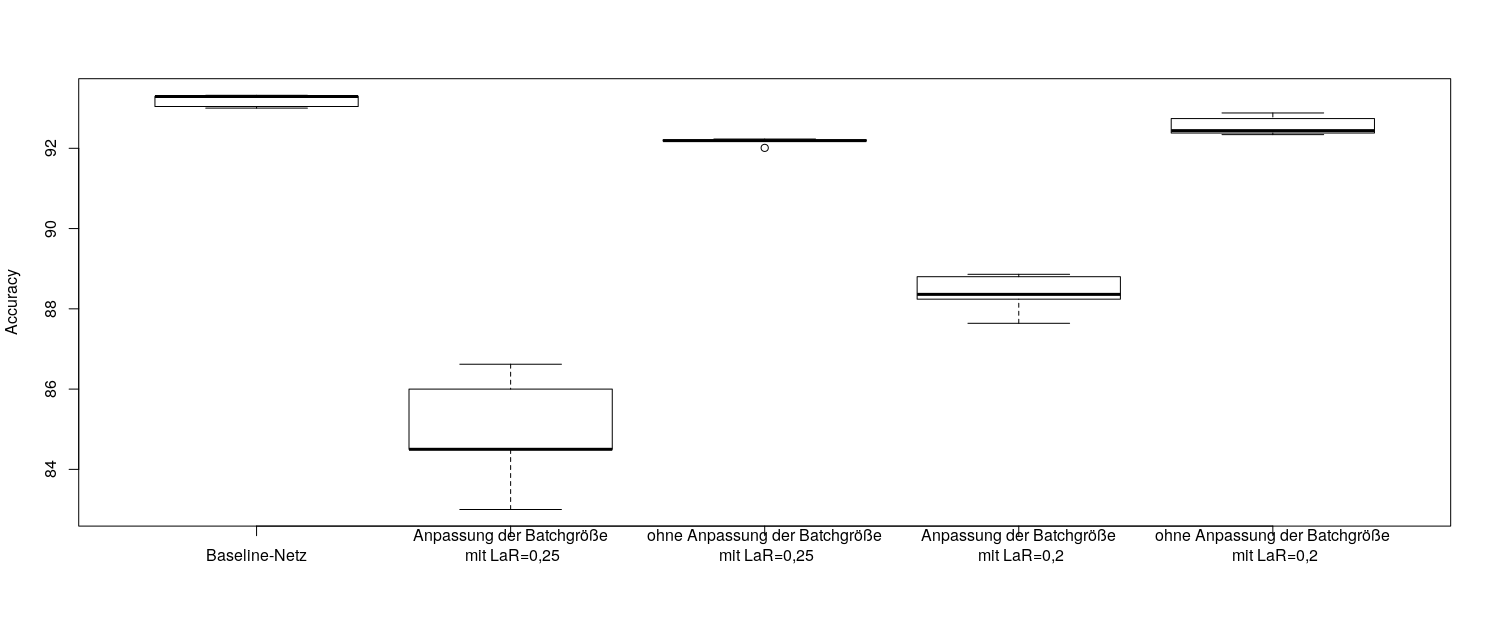
\includegraphics[width= .75\textwidth]{images/bSize2.png}\label{abb:bSize2}}\\
     \caption{Vergleich von (a) Durchschnittlicher Trainingszeit (b) Accuracys von PruneTrain mit Anpassung der Batchgrößeund Baseline-Netz}
     \label{abb:bSize}
\end{figure}
\end{frame}

\section{Net2Net}

\begin{frame}{Übersicht über Net2Net}
\begin{figure}[h]
 \centering
 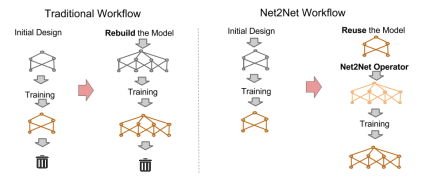
\includegraphics[width=0.8\textwidth]{images/net2net.png}
 % net2net.png: 433x179 px, 72dpi, 15.28x6.31 cm, bb=0 0 433 179
\end{figure}
\end{frame}

\begin{frame}{Evaluierung von Net2Net: Operator für ein breiteres Netz}
\begin{figure}
     \centering
     \subfloat[][]{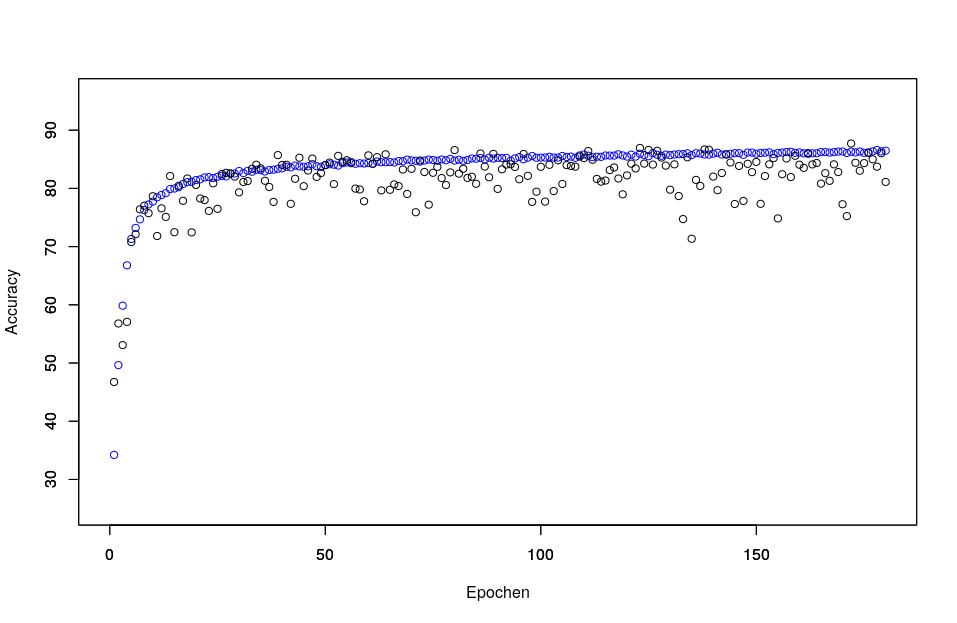
\includegraphics[width= .6\textwidth]{images/wider1.png}\label{abb:wider1}}     
\end{figure}
\end{frame}
     
\begin{frame}
\begin{figure}
     \subfloat[][]{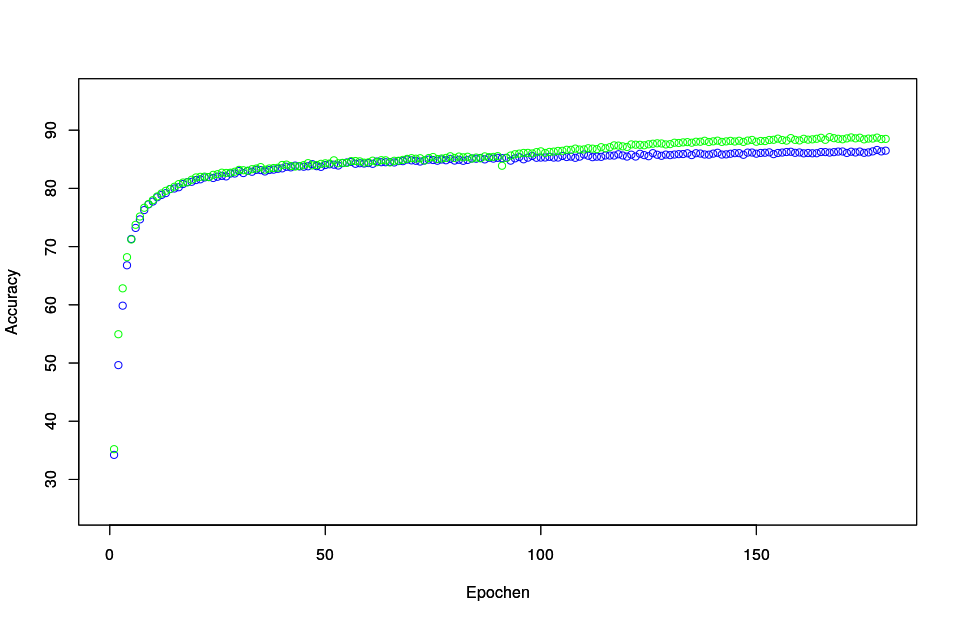
\includegraphics[width= .45\textwidth]{images/wider2.png}\label{abb:wider2}}
     \subfloat[][]{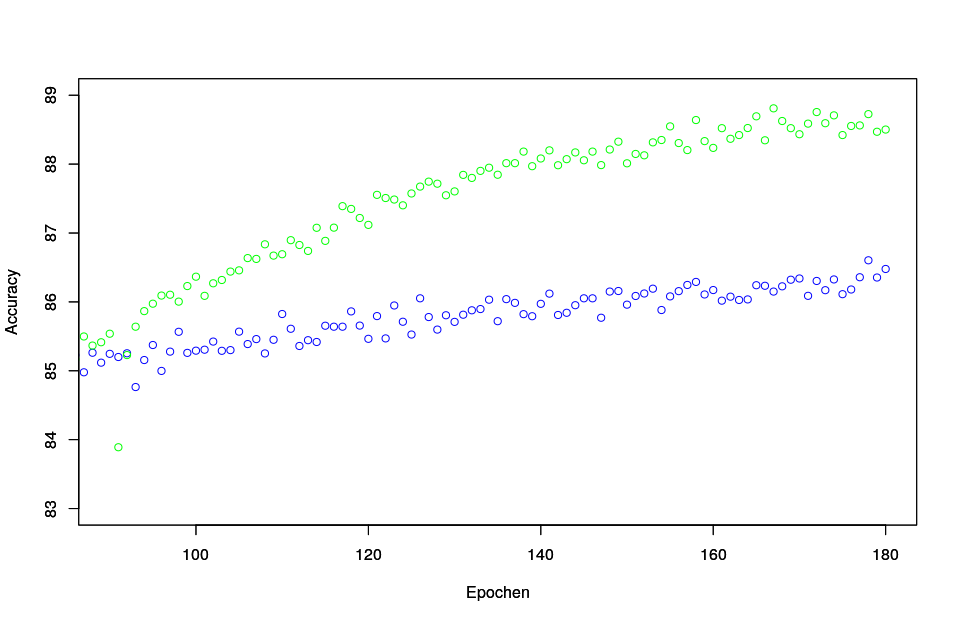
\includegraphics[width= .45\textwidth]{images/wider3.png}\label{abb:wider3}}
\end{figure}
\end{frame}

\begin{frame}
\begin{figure}
     \subfloat[][]{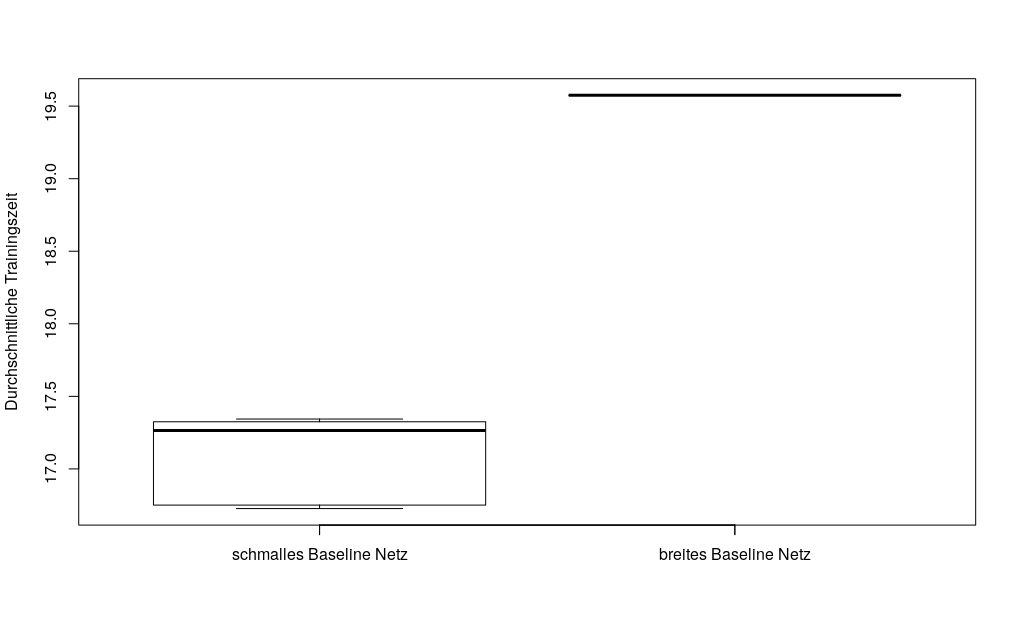
\includegraphics[width= .6\textwidth]{images/baselineS.png}\label{abb:wider4}}
     \caption{}
     \label{abb:wider}
\end{figure}
\end{frame}

\begin{frame}{Ergebnis der Evaluierung von Net2Net: Operator für ein tieferes Netz I}
 todo: Grafik für das Einfügen eines neuen Blocks
\end{frame}

\begin{frame}{Ergebnis der Evaluierung von Net2Net: Operator für ein tieferes Netz II}
\begin{figure}[h]
 \centering
 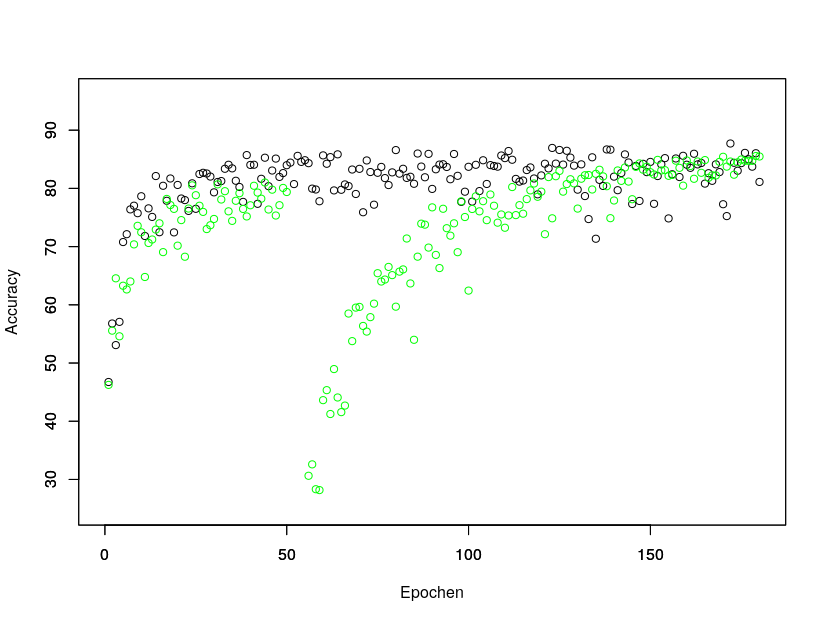
\includegraphics[width= 0.8\textwidth]{images/deeper14.png}
 % deeper14.png: 826x623 px, 96dpi, 21.86x16.49 cm, bb=0 0 620 467
\end{figure}



\end{frame}


\begin{frame}{Ausblick}

\end{frame}


\section{Anhang}

\begin{frame}{Architektur}
\end{frame}


\end{document}
